
\subsection{Flyback converter - CCM}
Der blev valgt en flyback converter opereret i CCM, som converter topologi i projektet. En sådan converter deles op i en primær- og en sekundær side. Primærsiden består af transformatorens primærvikling og et switch-element, der typisk er en MOSFET. Sekundærsiden består af transformatorens sekundærvikling en diode, en kondensator og udgangsbelastningen. En oversigt over den ideelle flyback converter er vist på figur~\ref{fig:flyabck_ideal}. 

\begin{figure}[H]
	\centering
	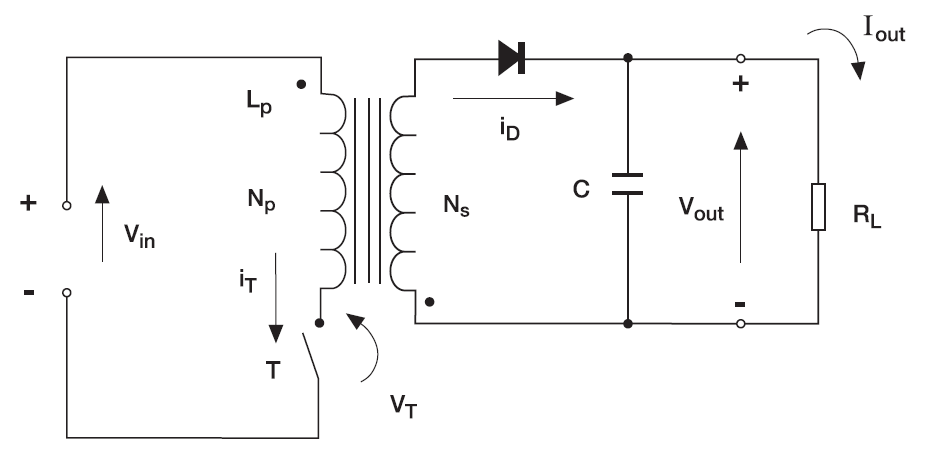
\includegraphics[width=0.7\linewidth]{../Dokumentation/tex/1iteration/billeder/flyback_ideal.png}
	\caption{Ideelt diagram for flyback converteren
		\cite{SMPS-topologies}}
	\label{fig:flyabck_ideal}
\end{figure}

Når MOSFET'en er ON, vil der være en positiv spænding over primærviklingen ved prikenden af viklingen, der er lig indgangsspændingen. Da denne spænding er positiv, vil det få strømmen i viklingen til at stige lineært over den tid MOSFET'en er ON. Strømændringen er bestemt ud fra formlen:
\begin{equation}
V = L \cdot \frac{di}{dt}
\end{equation}

Fordi polariteten af sekundærviklingen er modsat primærviklingen, vil dioden være forspændt i spærreretningen da kondensatoren vil opretholde udgangsspændingen over belastningen. Når dioden ikke kan lede strømmen fra sekundærviklingen, vil transformatoren oplagre energi i kernen når MOSFET'en er ON. Når MOSFET'en går OFF vil strømmen i viklingen ikke kunne skifte momentant. Det vil vende polariteten af transformatoren, så der nu er en positiv spænding diode enden af sekundærviklingen. Nu vil dioden være forspændt i lederetningen, og derfor lede den energi der er blevet oplagret i kernen, i form af en strøm. Den strøm vil nu holde den ønskede udgang, men også oplade kondensatoren, således den kan opretholde udgangsspændingen i næste ON-periode. Da der nu vil være en negativ spænding over sekundærviklingen ift. prikenden af den, vil strømmen i viklingen aftage i løbet af MOSFET'ens OFF periode på baggrund af den førnævnte formel. 

Kurveformen for strømmene i en flyback transformator er vist på figur~\ref{fig:flyabck_ideal_currents}. Her ses det der blev forklaret før. Når MOSFET'en er ON, vil strømmen i primærviklingen rampe op, mens strømmen i sekundærviklingen er 0. Når MOSFET'en er OFF vil strømmen i sekundærviklingen rampe ned fra det niveau primærstrømmen nåede, mens strømmen i primærviklingen nu vil være 0. Niveau-forholdet mellem strømmene i viklingerne, vil blive bestemt af viklingsforholdet i transformatoren. Skal converteren bruges til omsætning af store spændingsændringer fra indgang til udgang, kan dette bruges for at mindske tabet. 

\begin{figure}[H]
	\centering
	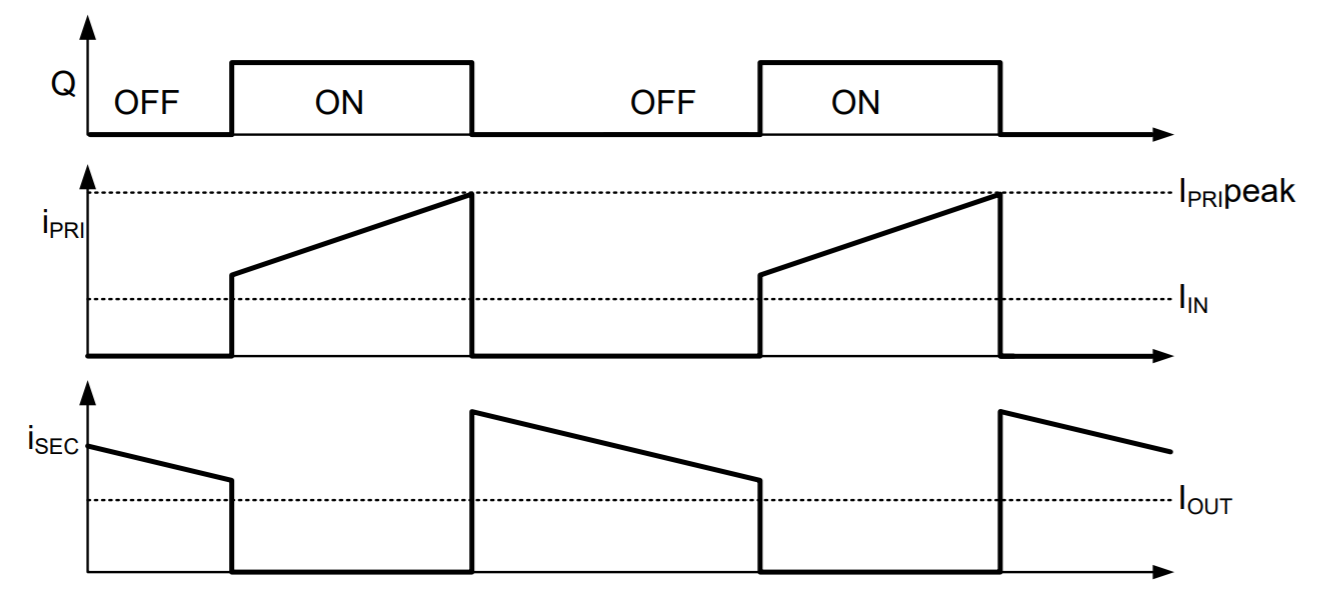
\includegraphics[width=0.7\linewidth]{../Dokumentation/tex/1iteration/billeder/CCM_transformer_current.png}
	\caption{CCM transformator strømme}
	\label{fig:flyabck_ideal_currents}
\end{figure}

selvom transformatoren i helhed opererer i CCM, vil strømmene i individuelt i viklingerne være diskontinuerte. Det betyder peak-strømmene i viklingerne bliver større for at kunne opretholde den ønskede udgangsstrøm. 

\noindent Overføringsfunktionen for flyback converteren i CCM er\cite{SMPS-topologies2}:
\begin{equation*}
	V_{out} = \frac{N_s}{N_p} \cdot \frac{D}{1-D} \cdot V_{in}
\end{equation*}

Da den mindste indgangsspænding og største udgangsspænding converteren skal designes efter næsten er ens, vælges det at tage udgangspunkt i en transformator en et viklingsforhold på 1. Ud fra dette, og intervallet på indgangsspændingen på $26-50V$, kan den maksimale duty-cycle regnes til $D_{maks} = 0.447$ eller $44.7\percent$, og den minimale duty-cycle renes til $0.296$ eller $29.6\percent$.  

Selvinduktionen i transformatorviklingerne bestemmes ud fra den ønskede ripple-strøm i transformatoren og den valgte switch-frekvens. Der er valgt at tage udgangspunkt i en switch-frekvens på $100k\hertz$. Når der er valgt at have et omsætningsforhold på 1, vil denne selvinduktion være gældende for begge viklinger. Selvinduktionen i transformatoren kan designes ud fra følgende formel\cite{flyback-formler}:
\begin{equation*}
	L = \frac{V_{inmin} \cdot D_{min}}{I_{ripple} \cdot f_s}
\end{equation*}

RMS-strømmene i viklingerne har stor betydning for det endelige tab i converteren. Derfor estimeres de i den indledende fase, for at vurdere betydningen af dette. RMS-strømmen i primærviklingen regnes til $3.02A$, og RMS-strømmen i sekundærviklingen regnes til $3.36A$. Begge er regnet ved en indgangsspænding på $26V$. 

Den ideelle converter er simuleret, for kontrol af dens funktionalitet. Figur~\ref{fig:flyabck_ideal_diagram} viser diagrammet for den ideelle converter. Her er der udelukkende fokuseret på transformatoren. Desuden er der indsat en kondensator på $223\micro F$, for at mindske ripple-spændingen på udgangen. Udgangen er blevet simuleret til det forventede $21V$ og $2.5A$, mens RMS-strømmene i transformatorviklingerne stemte overens med det beregnede. 

\begin{figure}[H]
	\centering
	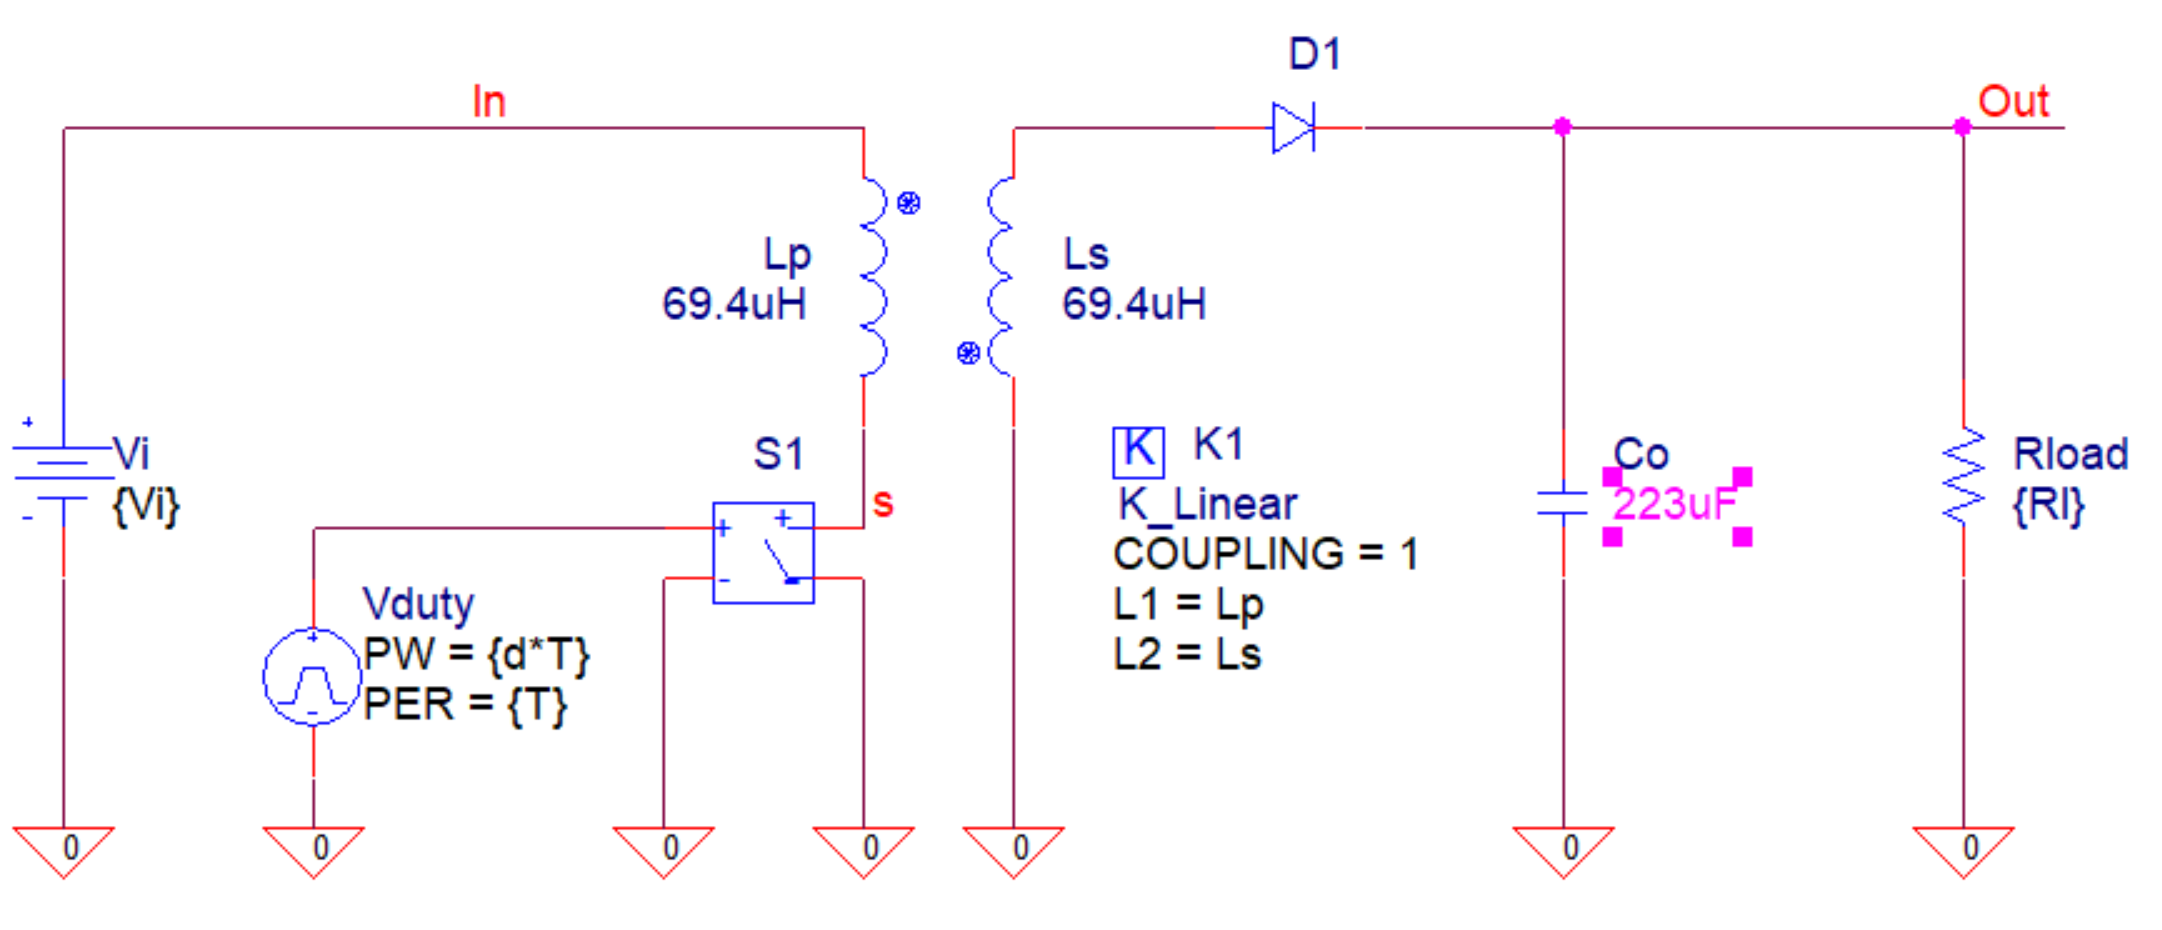
\includegraphics[width=0.7\linewidth]{../Dokumentation/tex/1iteration/billeder/flyback_ideal_diagram.png}
	\caption{Simulering af ideel flyback converter}
	\label{fig:flyabck_ideal_diagram}
\end{figure}

\noindent De præcise beregninger og simuleringer er beskrevet i dokumentationens afsnit 4.4.






